\documentclass[]{article}

\usepackage[T1]{fontenc} 
\usepackage{graphicx}
\usepackage{setspace}
\usepackage{amsmath}
\usepackage{geometry}
\usepackage{fancyhdr}
\usepackage{parskip}

% Page layout
\geometry{a4paper, margin=1in}

% Header and Footer
\pagestyle{fancy}
\fancyhf{}
\fancyhead[L]{\textbf{Werkzeuge für das wissenschaftliche Arbeiten}}
\fancyhead[R]{Python for Machine Learning and Data Science}
\fancyfoot[C]{\thepage}

\begin{document}


\vspace{1cm}
\begin{center}
    {\bfseries Abgabe: 15.12.2023}
\end{center}


\section*{Aufgabe 1}
In dieser Aufgabe beschäftigen wir uns mit Objektorientierung in Python. Der Fokus liegt auf der Implementierung einer Klasse, dabei nutzen wir insbesondere auch Magic Methods.

\begin{figure}[h!]
    \centering
    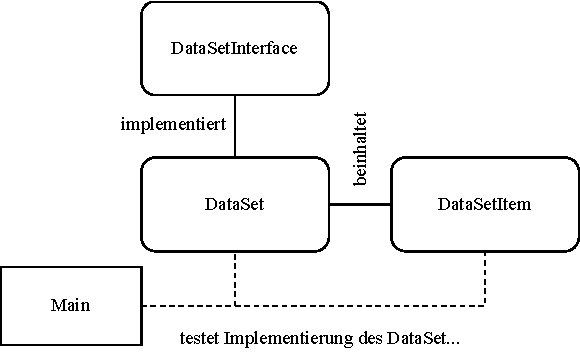
\includegraphics[width=12cm, height=5cm]{./../diagram/classes_files.pdf}
    \caption*{\small Abbildung 1: Darstellung der Klassenbeziehungen.}
\end{figure}

Ein Datensatz besteht aus mehreren Daten. Ein einzelnes Datum wird durch ein Objekt der Klasse \texttt{DataSetItem} repräsentiert. Jedes Datum hat einen Namen (Zeichenkette), eine ID (Zahl) und beliebigen Inhalt.

Nun sollen mehrere Daten, also Objekte vom Typ \texttt{DataSetItem}, in einem Datensatz zusammengefasst werden. Sie haben sich schon auf eine Schnittstelle und die benötigten Operationen, die ein Datensatz unterstützen muss, geeinigt. Es gibt eine Klasse \texttt{DataSetInterface}, die die Schnittstelle definiert und die Operationen jedes Datensatzes angibt. Bisher fehlt jedoch noch die Implementierung eines Datensatzes mit allen Operationen.

Implementieren Sie eine Klasse \texttt{DataSet} als eine Unterklasse von \texttt{DataSetInterface}.

Es gibt drei Dateien: \texttt{dataset.py}, \texttt{main.py} und \texttt{implementation.py}\footnote{https://github.com/ITI-WerkzeugeWissArbeiten/Git-2024-25/tree/main/code}
In der \texttt{dataset.py} befinden sich die Klassen \texttt{DataSetInterface} und \texttt{DataSetItem}, in der Datei \texttt{implementation.py} muss die Klasse \texttt{DataSet} implementiert werden. Die
Datei \texttt{main.py} nutzt die Klassen \texttt{DataSet} und \texttt{DataSetItem} aus den jeweiligen Dateien und testet die Schnittstelle und Operationen von \texttt{DataSetInterface}.

Bei der Klasse \texttt{DataSet} sind insbesondere folgende Methoden zu implementieren. Die genaue Spezifikation finden Sie in der Datei \texttt{dataset.py}:

\begin{enumerate}
    \item \texttt{\_\_setitem\_\_(self, name, id\_content)}: Hinzufügen eines Datums mit Name, ID und Inhalt.
    \item \texttt{\_\_iadd\_\_(self, item)}: Hinzufügen eines \texttt{DataSetItem}.
    \item \texttt{\_\_delitem\_\_(self, name)}: Löschen eines Datums basierend auf dem Namen. Der Name eines Datums ist ein eindeutiger Schlüssel und darf nur einmal pro Datensatz vorkommen.
    \item \texttt{\_\_contains\_\_(self, name)}: Prüfen, ob ein Datum mit diesem Namen im Datensatz vorhanden ist.
    \item \texttt{\_\_getitem\_\_(self, name)}: Abrufen des Datums über seinen Namen.
    \item \texttt{\_\_and\_\_(self, dataset)}: Schnittmenge zweier Datensätze bestimmen und als neuen Datensatz zurückgeben.
    \item \texttt{\_\_or\_\_(self, dataset)}: Vereinigung zweier Datensätze bestimmen und als neuen Datensatz zurückgeben.
    \item \texttt{\_\_iter\_\_(self)}: Iteration über alle Daten des Datensatzes (es ist möglich, eine Sortierung für die Reihenfolge der Iteration anzugeben).
    \item \texttt{filtered\_iterate(self, filter)}: Gefilterte Iteration über einen Datensatz. Eine Lambda-Funktion mit den Parametern Name und ID dient als Filter.
    \item \texttt{\_\_len\_\_(self)}: Abrufen der Anzahl der Daten in einem Datensatz.
\end{enumerate}

\section*{Abgabe}
Programmieren Sie die Klasse \texttt{DataSet} in der Datei \texttt{implementation.py} zur Lösung der oben beschriebenen Aufgabe im VPL. Sie können auch direkt auf Ihrem Computer programmieren. Dazu finden Sie alle drei benötigten Dateien zum Download im Moodle.

Das VPL nutzt denselben Code. Die Datei \texttt{main.py} wurde jedoch um weitere Testfälle und Überprüfungen erweitert. Diese Überprüfungen dienen dazu, sicherzustellen, dass Sie die richtigen Klassen nutzen.


\end{document}